% This file is part of the stream_information project.
% Copyright 2017 the authors. All rights reserved.

% # style notes
% - it is Cram\'er--Rao not Cram\'er-Rao. And yet Fisher-matrix not Fisher--matrix.

\documentclass[modern]{aastex61}

% typography
\setlength{\parindent}{1.\baselineskip}
\newcommand{\acronym}[1]{{\small{#1}}}
\newcommand{\CRLB}{\acronym{CRLB}}
\newcommand{\FF}{\texttt{FAST FORWARD}}

% aastex parameters
%%\hypersetup{linkcolor=red,citecolor=green,filecolor=cyan,urlcolor=magenta}
\received{not yet; THIS IS A DRAFT}
%\revised{not yet}
%\accepted{not yet}
%% Adds "Submitted to " the arguement.
%\submitjournal{ApJ}
\shorttitle{information in stellar streams}
\shortauthors{bonaca et al.}

\usepackage{amsmath}

\begin{document}\sloppy\sloppypar\raggedbottom\frenchspacing % trust me

\title{The information content in cold stellar streams}

\correspondingauthor{Ana Bonaca}
% \email{whatevs}

\author[0000-0002-7846-9787]{Ana Bonaca}
\affil{Harvard--Smithsonian Center for Astrophysics}

\author[0000-0003-2866-9403]{David W. Hogg}
\affiliation{Center for Cosmology and Particle Physics,
Department of Physics,
New York University}
\affiliation{Center for Data Science,
New York University}
\affiliation{Flatiron Institute, Simons Foundation}
\affiliation{Max-Planck-Institut f\"ur Astronomie, Heidelberg}

\begin{abstract}\noindent % trust me
Cold stellar streams---produced by tidal disruptions of globular
clusters (or equivalent)---are long-lived, coherent dynamical features
in the stellar halo of the Milky Way.
They have delivered precise information about the mass distribution or
gravitational potential, including constraints on the shape of the
dark-matter halo.
Because of their different positions in phase space, different ages,
and different levels of observational scrutiny, different streams tell
us different things about the Galaxy.
Here we employ a Cram\'er--Rao (\CRLB) or Fisher-matrix approach to
understand the quantitative information content in the known
streams (Pal5, GD-1, Styx, [full list here]).
This approach depends on the existence of a generative model of
stellar streams, which we have developed previously, and which permits
easy calculation of derivatives of predicted stream properties with
respect to Galaxy model parameters.
We find that, in simple, static, analytic models of the Milky Way,
streams XX and YY contain the most information about the dark-matter
shape.
For any individual stream, there are near-degeneracies between
dark-matter halo properties and other parameters, including the mass
of the Large Magellanic Cloud, the total dark-matter mass, and other
potential parameters, but we find that simultaneous fitting of multiple
streams ought to precisely constrain all parameters well.
The \CRLB\ on any one parameter depends strongly on the model freedom;
as we permit more potential freedom, the information about, say, halo
triaxiality, reduces.
We perform experiments to demonstrate this using potential basis
functions that permit great freedom in the gravitational potential on intermediate
scales.
The \CRLB\ formalism also permits us to assess the value of future
measurements of stellar velocities, distances, and proper motions. We
make some comments about the information value of various new
observations that could be made of particular known streams.
\end{abstract}

\keywords{foo --- bar --- hello --- world}

\section{Introduction} \label{sec:intro}

\begin{itemize}
 \item establish streams useful in constraining gravitational potential
 \item tied to parametric models (too complex for inference otherwise, at least in current approaches)
 \item constraints only as good as the model (VL2 results)
 \item so, since not likely that the true potential is NFW, what are the streams actually constraining? 
 \item here we're building a framework to measure the information content of stellar streams regarding the gravitational potential
 \item two-fold goals: given a simple parametric model, what kind of data do we need? what aspect of a (non-parametric) potential do individual streams constrain?
\end{itemize}


\section{Methods}
\label{sec:method}

\subsection{Information content in stellar streams}
Numerous methods have been developed to estimate properties of a dark matter halo by modeling observations of stellar streams \citep[e.g.,][]{}.
In this approach, the dark matter halo is usually described by an analytic model with a handful of free parameters.
We define the information content in this context as the best-case uncertainties on our model parameters achievable using the observational data at hand.
Formally, the lower bound on the variance of a deterministic parameter is given by the Cram\' er--Rao lower bound \citep[\CRLB,][]{Cramer1946, Rao1945}.

For some data set $\vec{y}$ (e.g., a vector of position and velocity measurements of stars along a stream), the associated covariance matrix is $C_y$.
Given the model parameters $\vec{x}$ (e.g., a vector with the mass and scale radius of a dark matter halo), the Cram\' er--Rao bound is the covariance matrix $C_x$.
The \CRLB\ is set by the inverse of a Fisher information matrix \citep{}:
\begin{equation}
C_x^{-1} = \left(\frac{d\vec{y}}{d\vec{x}}\right)^{T} C_y^{-1} \left(\frac{d\vec{y}}{d\vec{x}}\right) + V_x^{-1}
\label{eq:crlb}
\end{equation}
where $V_x$ is a covariance matrix containing the prior knowledge of model parameters.
In the next two subsections, we describe individual terms of Equation~\ref{eq:crlb}: model and its existing constraints (\S\ref{sec:model}), the change in stream observables $\vec{y}$ as a function of changes in the gravitational potential $\vec{x}$, i.e., the derivative $d\vec{y}/d\vec{x}$ (\S\ref{sec:derivatives}), and the adopted observational uncertainties, which set the covariance matrix $C_y$ (\S\ref{sec:datasets}).

\subsection{Model definition}
\label{sec:model}
The \CRLB\ formalism can only quantify information in the context of a model, which in our case is a model of a stellar stream in the gravitational potential of the Milky Way.
We consider cold stellar streams originating from disrupting globular clusters, which have been well-modeled with direct N-body simulations (refs).
These studies have shown that the phase-space distribution of the resulting debris is predominantly set by properties of the gravitational potential and the orbit of the progenitor, with a weaker dependence on the internal properties of the progenitor.
Hence, our model consists of parameters defining the gravitational potential and a 6-dimensional position of the progenitor.

To represent the global properties of the Milky Way, we represent the gravitational potential as a combination of a Hernquist bulge (parameterized with mass and scale radius), a Miyamoto-Nagai disk (with parameters for disk mass, scale length and scale height) and a spherical NFW halo (parameterized with scale velocity, scale radius, and axis ratios $q_x=q_z=1$).
We provide the fiducial values for this model in Table~\ref{t:model}, along with measurement uncertainties where available.
This potential is similar to MWPotential2014 \citep{galpy}, and fits a range observed Milky Way properties (e.g., rotation curve, ..., cit).

Next, we search for globular cluster orbits in the fiducial gravitational potential that produce stellar streams similar to those observed in the Milky Way.
Briefly, we use the streakline method to forward-model stream observations in a modification of the \FF\ framework from \citet{bonaca2014}.
For each stream, we vary the properties of its progenitor, while keeping the potential fixed at fiducial values.
Observations of all streams consist of on-sky positions of likely members, and their distance estimates from the location in the color-magnitude diagram.
Some streams have been better characterized, for example, with radial velocities from follow-up spectroscopy, and we include these extra dimensions of data in the parameter search if they are available.
In Appendix~\ref{sec:streams}, we provide current progenitor positions, initial masses and stream ages, which reproduce observations for most of the Galactic streams present in the PanSTARRS1 footprint, as well as more details on the above procedure.
When calculating the \CRLB\ for streams, we keep the progenitor mass and age fixed at their best-fitting values, as they are highly degenerate, and only use the present-day position of the progenitor as model parameters (defined in the observable space with the progenitor's two on-sky position angles, distance, radial velocity and two proper motion components). 

The complete model for measuring the information content in stellar streams has 15 parameters: nine for the distribution of matter in the Galaxy and six for the position of the stream progenitor (as defined in Table~\ref{t:model}).
Some of these parameters have already been measured, and we include these prior constraints as appropriate. 
For example, progenitors of streams are generally unknown, but several have been identified, such as globular clusters Palomar~5 and NGC~5466, and we include observational uncertainties on their position in our analysis through covariance matrix $V$ in Equation~\ref{eq:crlb}.
A substantial body of work has already been dedicated to constraining the mass components of the Milky Way.
As a result, properties of the bulge and the disk are known with a precision of x\% (cit) (from different kinds of study too?), which we include in covariance matrix $V$.
The halo mass, however, is still uncertain up to a factor of a few (cits), and the reported constraints on the halo shape are conflicting (cit), so the information that streams provide on the dark matter halo we measure independently of prior work.

\begin{center}
\begin{table}
\begin{tabular}{l c c c l}
\hline
\hline
Parameter & Symbol & Fiducial value & Uncertainty & Reference \\
\hline
\hline
Bulge mass & $M_b$ & & & \\
Bulge scale radius & $a_b$ & & & \\
Disk mass & $M_d$ & & & \\
Disk scale radius & $a_d$ & & & \\
Disk scale height & $b_d$ & & & \\
\hline
Halo scale velocity & $V_h$ & & & \\
Halo scale radius & $R_h$ & & & \\
Halo $y$ axis ratio & $q_y$ & & & \\
Halo $z$ axis ratio & $q_z$ & & & \\
\hline
Progenitor RA & $RA_p$ & & & \\
Progenitor Dec & $Dec_p$ & & & \\
Progenitor distance & $d_p$ & & & \\
Progenitor radial velocity & $V_{r,p}$ & & & \\
Progenitor RA proper motion & $\mu_{\alpha,p}$ & & & \\
Progenitor Dec proper motion & $\mu_{\delta,p}$ & & & \\
\hline
\hline
\end{tabular}
\caption{Model parameters}
\label{t:model}
\end{table}
\end{center}

\subsection{Calculating numerical derivatives for the \CRLB}
\label{sec:derivatives}
Intuitively, CRB is quantifying how much we can change the parameters of a model, without violating the observational uncertainties of our data
- to calculate this, we need the inverse of how much observed quantities vary as a function of model parameters, or formally the derivative $d\vec{y}/d\vec{x}$.
- non-trivial when our data is a collection of points in a 6-dimensional space ( Stellar streams are characterized by positions and velocities of their member stars, so their observed quantities are on-sky positions, distances, radial velocities and proper motions.)
- using the streakline method \citep{bonaca2014}
- timestep: tested time step small enough so that we're not introducing numerical noise that way
In what follows, we describe how we measure differences in stream models of different input parameters.

\begin{figure}
\begin{center}
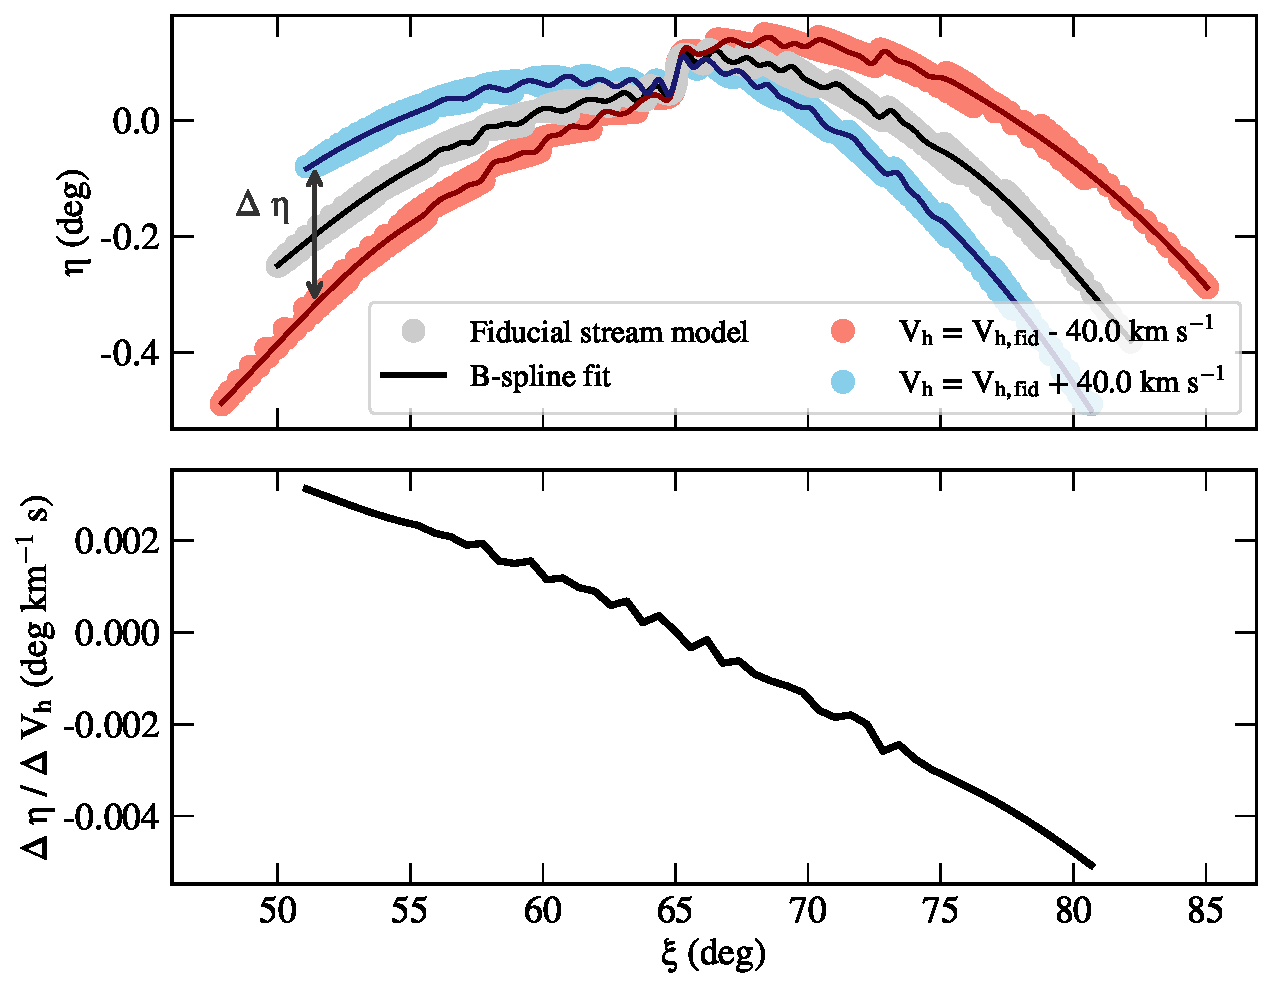
\includegraphics[width=0.8\textwidth]{derivative_vis.pdf}
\caption{We quantify the response of streams on changes in model parameters by calculating numerical derivatives, and in this figure we visualize the $d\eta / d V_h$ derivative (change in the sky position with the change in scale velocity of the underlying dark matter halo).
(\emph{Top}) The on-sky positions of the fiducial stream are shown in gray points, while the colored points show models in a less massive (red) and more massive halo (blue).
Solid lines show B-spline fits through these stream models.
The coordinate system is rotated such that the $\xi$ coordinate is approximately along the fiducial stream model, and $\eta$ is perpendicular to this stream track. 
(\emph{Bottom}) We define the derivative $d\eta / d V_h$ as the numerical derivative $\Delta\eta / \Delta V_h$.
At a fixed coordinate $\xi$ along the stream, the numerical derivative is the ration of the difference between $\eta$ coordinates of models in the more massive and the less massive halo ($\Delta\eta$, marked with arrows in the top panel), and the total difference in halo scale velocity between these two models ($\Delta V_h$).
This numerical derivative as a function of position along the stream is shown in a black line on the bottom panel.
}
\label{fig:derivative_steps}
\end{center}
\end{figure}

Figure~\ref{fig:derivative_steps} outlines major steps in our calculation of the numerical derivatives.
We start by creating a pair of stream models, where we change parameter $x_i$ to $x_i = x_{i,0} \pm \Delta x_i$, and keep the rest of the parameters at their fiducial values, $x_j = x_{j,0}$ for $j\neq i$.
The first row of Figure~\ref{fig:derivative_steps} shows models of the GD-1 stream with different offsets $\Delta V_{h}$ from the fiducial scale velocity (color-coded such that the positive offsets are in shades of red, and negative in shades of blue).
Each observable is shown as a function of longitudinal position along the stream, $\xi$, in a separate column in the order from left to right: transverse on-sky position, $\eta$, distance, $d$, radial velocity, $V_r$, and the two proper motion components, $\mu_{\alpha*}$ and $\mu_\delta$.
For each stream, the on-sky positions are rotated to a system in which the great circle best-fitting of the stream track is on the equator.
We describe how we fit these great circles, and provide rotation matrices from the equatorial system to the stream coordinates in Appendix~\ref{sec:streams}.
Stream models with different scale velocities appear different in all of the observables.
To highlight these differences, we show deviations from the fiducial stream track in the second row.


- the derivative: at fixed stream longitude, $\xi_i$, difference the observable in two models, $\Delta y|_{\xi_i}$.
- regard only transverse direction, as longitudinal has a strong degeneracy with stream age
- noisy data due to the particle nature of streams, interested in a general shape of the stream, so we're fitting a bspline to the stream (more stable than polynomial)
- difference of bsplines from the fiducial for different step sizes in third row
- difference of bsplines divided by the step size in fourth row -- small steps have larger deviations, but these derivatives agree at larger step sizes
To be more robust, we define the derivative of observable $y_i$ with respect to model parameter $x_i$ using symmetrical offsets from the fiducial model:
\begin{equation}
\left.\frac{d y_i}{d x_j}\right\rvert_{\xi_k} = \left.\left(\frac{y_i(x_{0,j} + \Delta x_j) - y_i(x_{0,j} - \Delta x_j)}{2\Delta x_j}\right)\right\rvert_{\xi_k}
\label{eq:derivative}
\end{equation}
for an observation made at the longitudinal position $\xi_k$.
Thus defined derivatives are shown in the last row of Figure~\ref{fig:derivative_steps}, with darker colors corresponding to larger step sizes.
- good agreement

\begin{figure}
\begin{center}
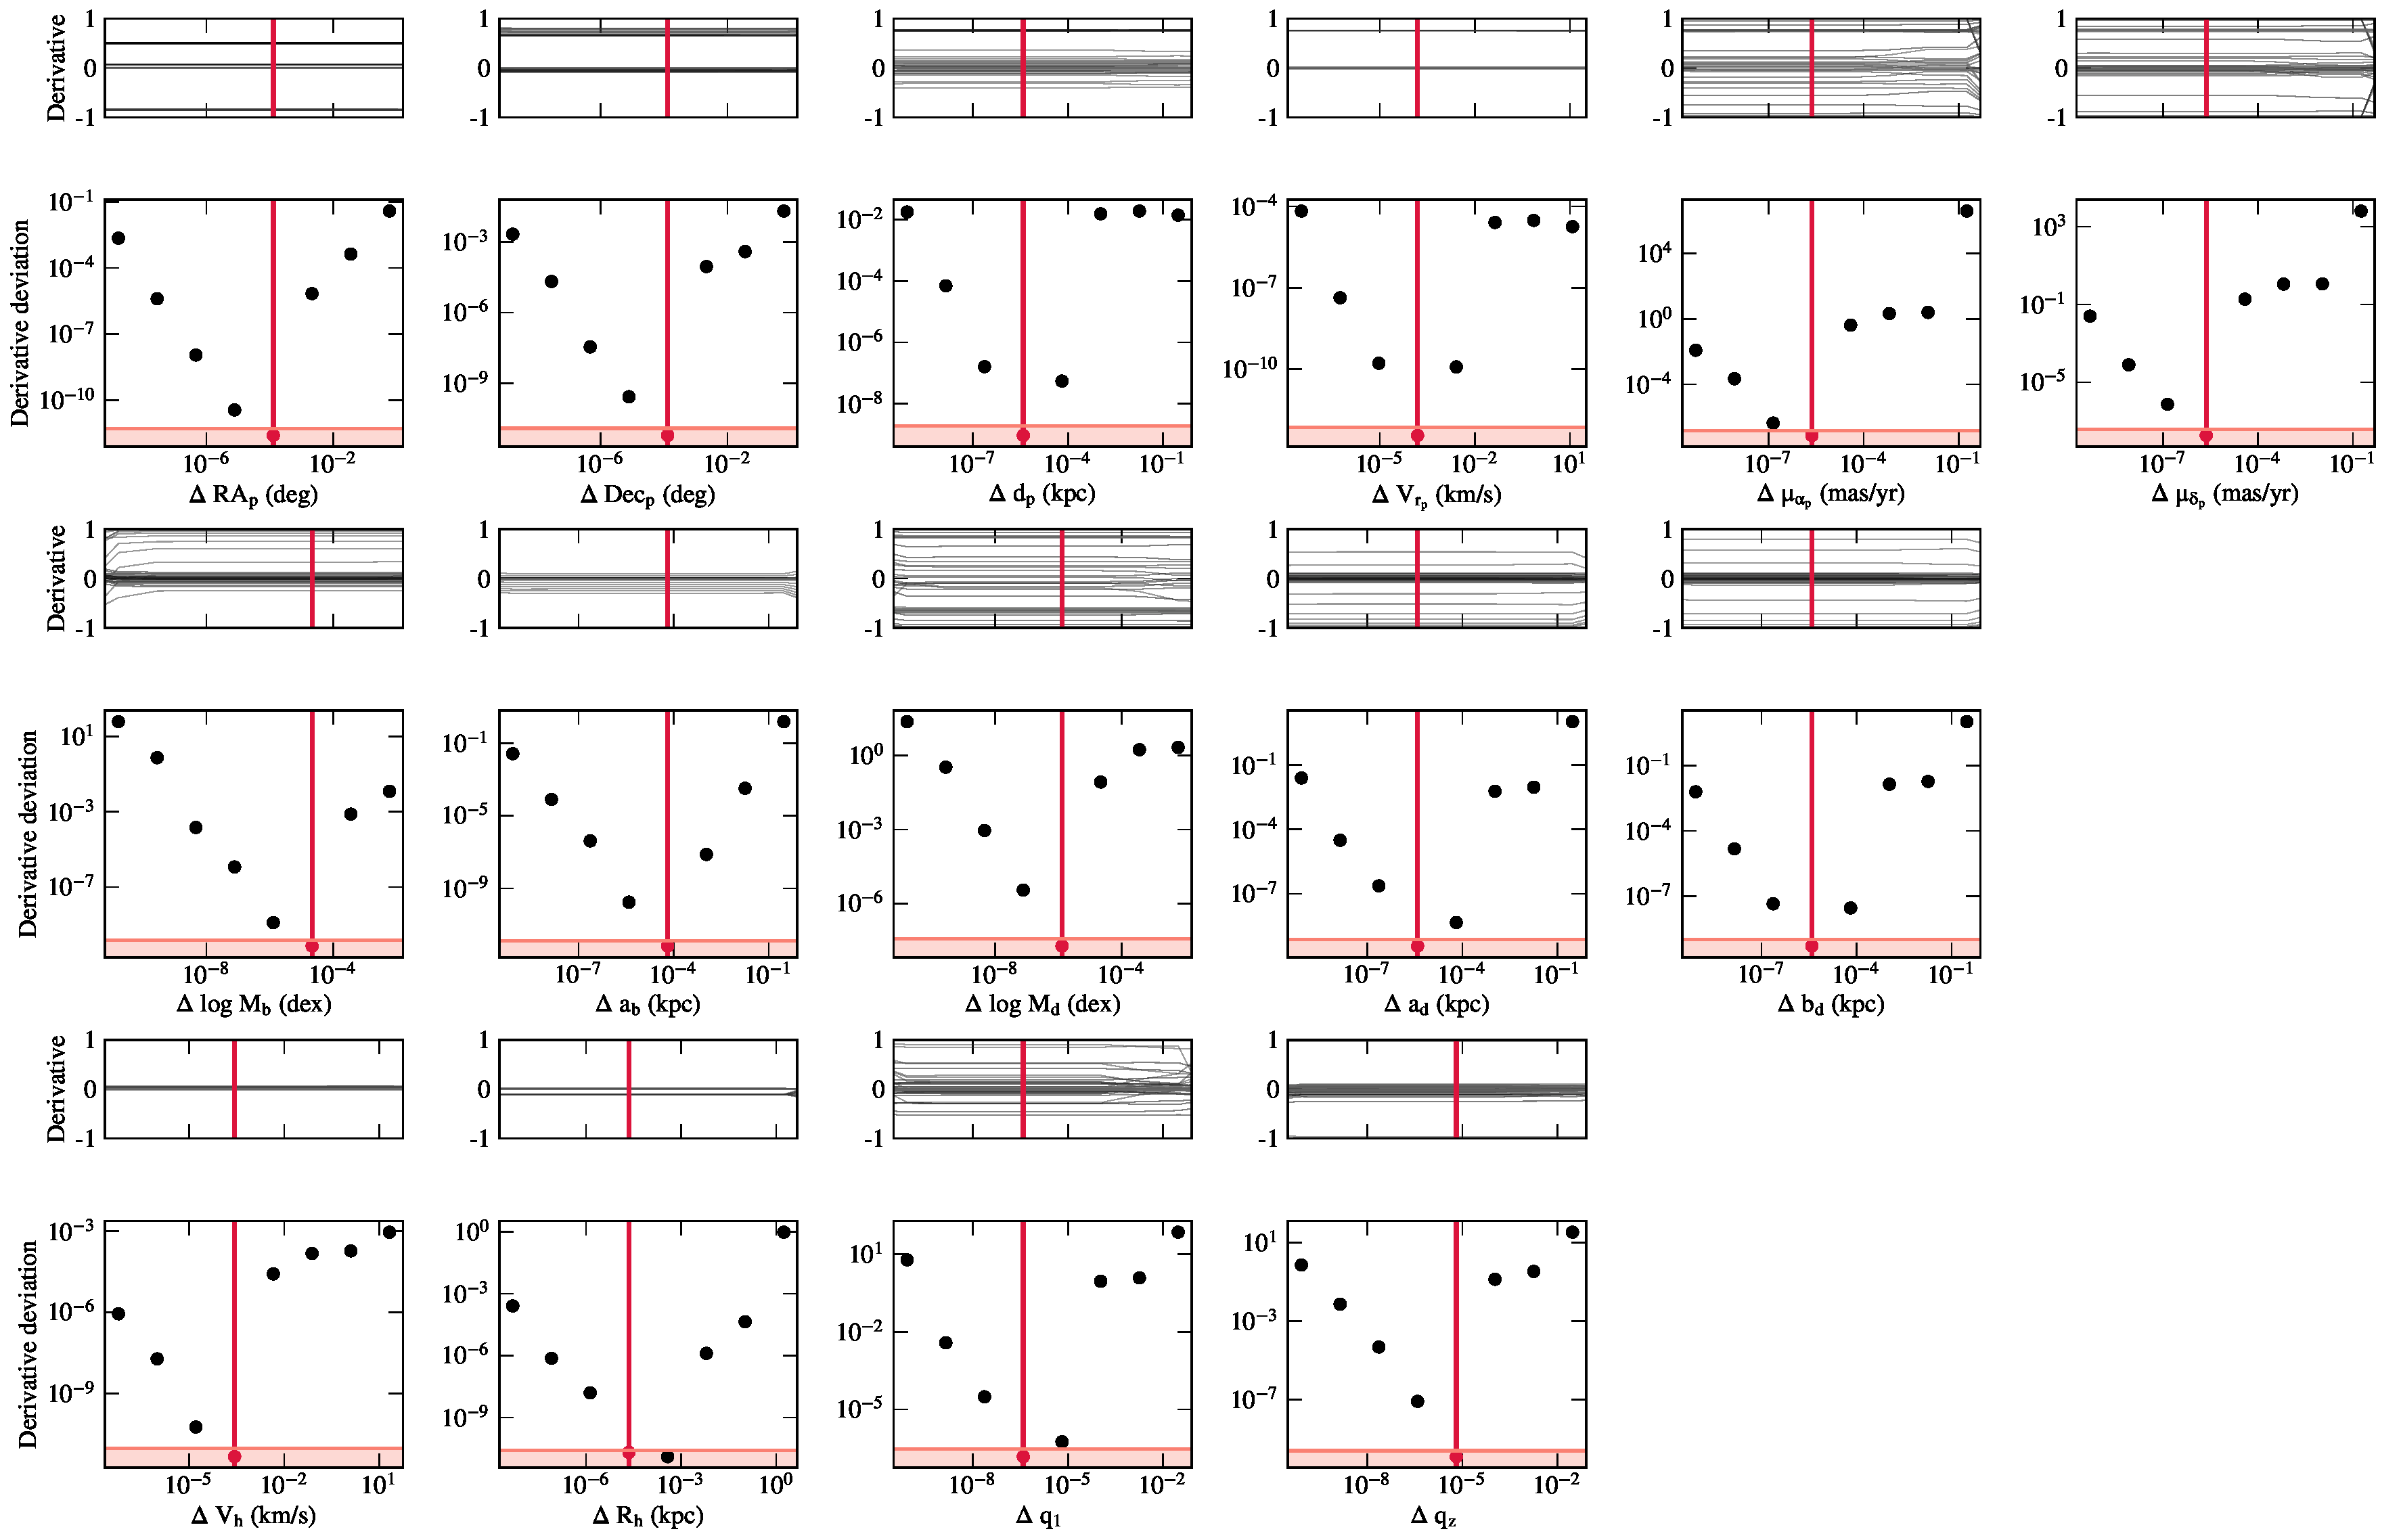
\includegraphics[width=\textwidth]{derivative_steps.pdf}
\caption{Optimal steps in parameter space for calculating numerical derivatives are marked with red vertical lines.
The top two rows present progenitor parameters, starting with progenitor position, $\rm RA_p$, on the left, until progenitor proper motion $\mu_p$ on the right.
The first of these two rows shows the values of evaluated numerical derivative, $\Delta y/\Delta x$, as a function of step size for parameter $x$ used in calculation, $\Delta x$, and the second row shows how the derivatives along the stream observables evaluated at a step size $\Delta x_j$ deviate from derivatives at adjacent step sizes $\Delta x_{j-1}$ and $\Delta x_{j+1}$.
Similarly, the middle two rows present derivatives for parameters defining the bulge and the disk, while the bottom two rows are dedicated to parameters of the dark matter halo.
For all of the model parameters, there is a local minimum in derivative deviation.
We adopt the optimal step size (red points and vertical lines) as the smallest step with a derivative deviation within a factor of 2 from the local minimum.
}
\label{fig:derivative_conv}
\end{center}
\end{figure}

- to quantify whether these have converged
- choice of step size for numerical derivative such that the derivative converged

\subsection{Sets of observational data}
\label{sec:datasets}

\begin{table}
\begin{center}
\begin{tabular}{l c c c c c c}
\hline
\hline
Data set & $\sigma_\alpha$ & $\sigma_\delta$ & $\sigma_d$ & $\sigma_{V_r}$ & $\sigma_{\mu_\alpha}$ & $\sigma_{\mu_\alpha}$ \\
\hline
Fiducial & & & & & & \\
DESI & & & & & N/A & N/A \\
Gaia & & & & & & \\
Extragalactic & & & N/A & & N/A & N/A \\
\hline
\hline
\end{tabular}
\caption{Observational data sets}
\label{t:datasets}
\end{center}
\end{table}

We measure the information content in the Milky Way streams as currently observed, and also quantify improvements expected from the upcoming observational campaigns.
In total, we consider three classes of observational data:
\begin{enumerate}
\item fiducial data set with data obtainable at the present,
\item including present data on positions of stream stars with radial velocities from DESI and DESI-like surveys,
\item data on stream members from the final data release from the Gaia mission, and
\item integrated-light data on extragalactic streams.
\end{enumerate}
Observational uncertainties in each of these cases are summarized in Table~\ref{t:datasets}, which we describe in more detail below.

In the fiducial data set, we assume that the positions of stream members come from photometric surveys, radial velocities from targeted spectroscopic follow-up, and proper motions from long-baseline, spacecraft observations.
- on-sky positions uncertain by the width of the stream, typically x deg (cit)
- distances from msto position, uncertain to x \% (cit)
- a number of medium-resolution spectrographs have demonstrated radial velocities measured to 1\,km/s level (cit), which we adopt
- HST measurements of proper motions for individual members of the Sgr stream were typically uncertain by 0.1\,mas/yr
- these uncertainties, especially for the kinematic data, are currently best attainable
- most of the streams, however, only have positional data, and a few have kinematic information from radial velocities
- so within the fiducial case, we consider separate situations of having access to 3D, 4D and 6D data

- second case, we consider data on positions from photometric surveys, same as in the fiducial case, but with velocities from lower resolution, but large scale spectroscopic surveys
- a number of such surveys (cit) are about to launch, with the expected uncertainty of 10\,km/s in radial velocity of a g=20 star
- albeit an order of magnitude worse precision, we consider this case for its potential to provide kinematics for all of the known streams, and potentially many fainter stream discoveries. 

Our final case studies data in the post-Gaia era, where the distances come from Gaia parallaxes, radial velocities from RVS, and proper motions from the 5 year Gaia astrometry.
- stream positions still limited by their intrinsic width, but the distance is improved an order of magnitude wrt the fiducial case (cit typical Gaia parallax uncertainty)
- streams far away, so we adopt RVS performance for faintest stars of x\,km/s
- similarly, proper motion precision is x\,mas/yr for faint, blue stars, such as those at the main sequence turn-off of stellar streams.

For simplicity, we assume that there are 50 observations uniformly distributed along the length of each stream, and also that the uncertainties are the same for all of the observations.
As there are density inhomogeneities along the streams, the likely members are hardly equidistant.
Furthermore, realistic observational uncertainties are a function of stellar brightness, color, and often distance.
However, the idealized scenario adopted here serves as a demonstration for the framework of calculating the information content of a stream data set.
More realistic data can be analyzed in the same way to produce specific predictions.

\section{Results}

\subsection{Individual stream}
- covariances
- triangle plot

% \begin{figure}
% \begin{center}
% 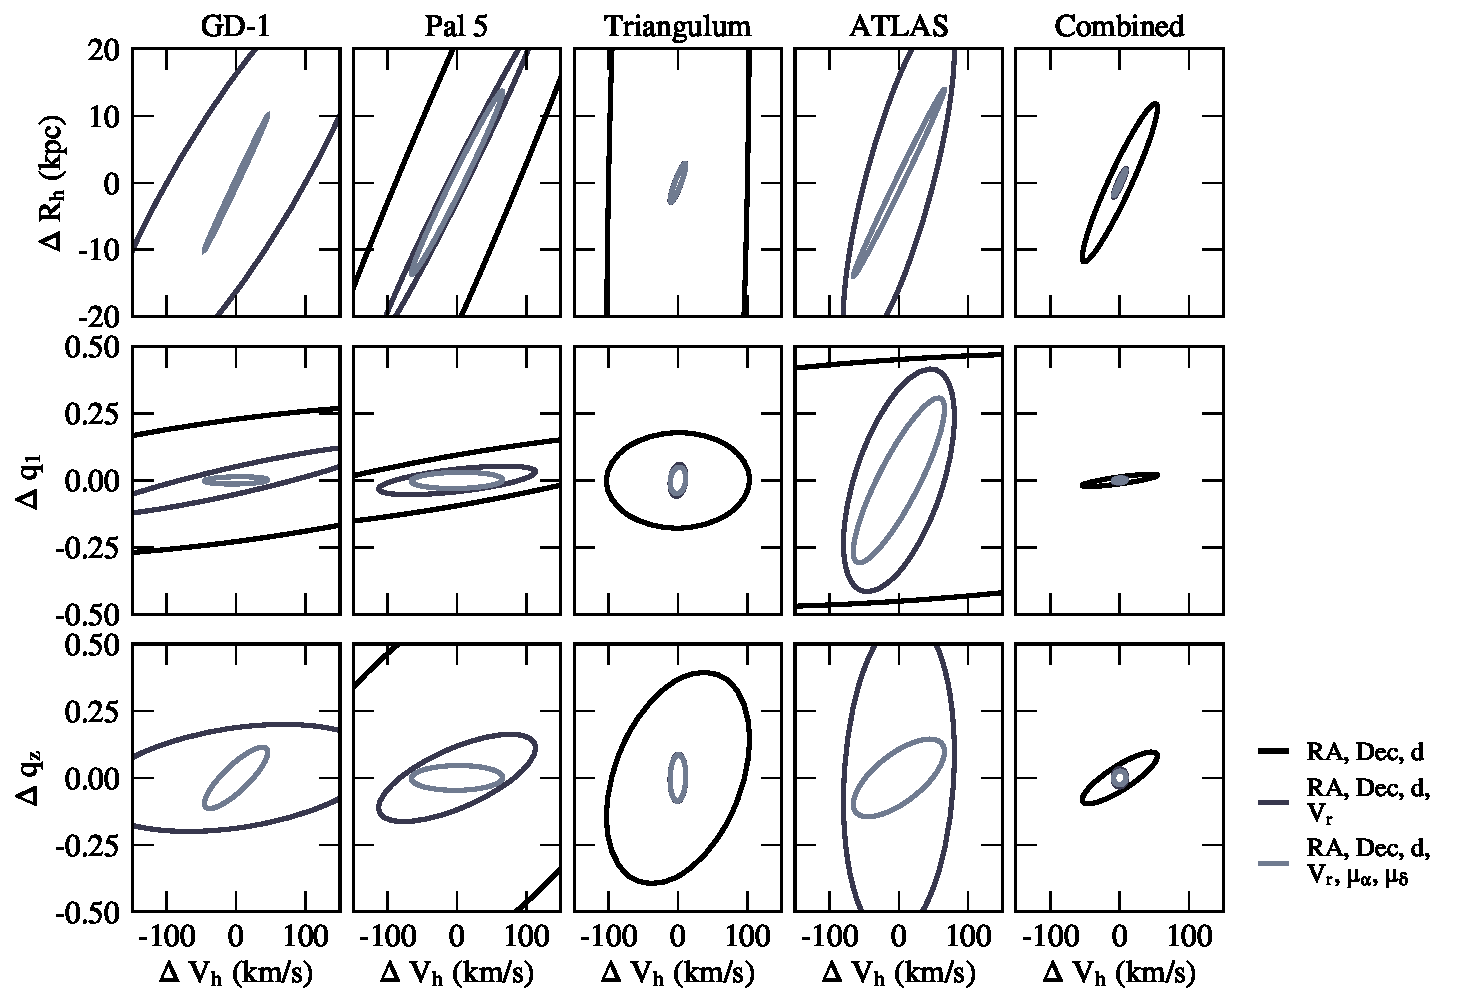
\includegraphics[width=\textwidth]{crlb_2d.pdf}
% \caption{Two-dimensional Cram\' er--Rao lower bounds that cold stellar streams put on parameters of the Milky Way dark matter halo.
% Parameters considered are the halo scale velocity $V_h$, scale radius $R_h$, $x/y$ and $z/y$ axis ratios $q_1$ and $q_z$, respectively.
% Parameter combination is the same across the rows.
% Bounds based on individual streams (GD-1, Pal~5, Triangulum and ATLAS) are shown in the first four columns, and their combination is presented in the last column.
% The ellipse color denotes the dimensionality of the observational data used to calculate the bound; the darkest ellipses are based on positional information only, medium-colored ellipses include positions and radial velocity, and the lightest ellipses are derived using the full 6-D phase space of streams.
% Not all streams are equally constraining for all of the parameters, but for a given stream, parameter constraints improve when more phase-space dimensions are included.
% Combining different streams results in the most precise recovery of the halo parameters.
% Even if only limited observational data is available for multiple streams, the obtained bounds are comparable to, or better than, the best bounds coming from any individual stream.
% }
% \label{fig:2dbounds}
% \end{center}
% \end{figure}

\subsection{Comparison between streams}
- compare CRB ellipses for halo parameters between several streams

\subsection{Joint constraints}
- CRB on halo parameters using different combinations of streams

\subsection{Different observing modes}


\section{Discussion}

\subsection{Physical interpretation of constraints}
- enclosed mass
- flattening

\subsection{More flexible potential models}

% \subsubsection{LMC}

\subsubsection{Basis function expansion}



\emph{Acknowledgements:} This work was improved upon following the thoughtful suggestions of Dan Foreman-Mackey, Kathryn Johnston, Nikhil Padmanabhan and Hans-Walter Rix, and it is a pleasure to thank them.

\bibliographystyle{aasjournal}
\bibliography{crlb}

\appendix
\section{Cold tidal streams in the Milky Way}
\label{sec:streams}

Steps for creating a mock stream:
\begin{itemize}
 \item obtain ridge points along the stream. This is done either by analyzing a match-filtered map showing the stream, or from published stream tracks (usually in a polynomial form).
 \item fit a polynomial to the ridge points, and define a stream coordinate system with one axis along the polynomial, and the other along the normal on the polynomial.
 \item query PanSTARRS1 star catalog and assign a membership probability. We assume that the total probability can be split in a spatial and color-magnitude component; $p = p_{spatial} \times p_{CMD}$. The spatial probability follows a normal distribution centered on the stream track (measured as described above), with dispersion matching the reported stream width. The color-magnitude probability is obtained from a matched filter based on the M13 globular cluster, and placed at the reported distance to the stream.
 \item select a hundred most likely members. If kinematic information is present, the lowest probability members are replaced by stars with kinematic measurements.
 \item these hundred members are then used to constrain parameters of the mock stream progenitor. The mock stream is created in a fiducial gravitational potential defined by the first 9 parameters listed in Table~\ref{t:model} and these parameters are kept fixed for all of the mock streams. The variable parameters are: 6D position of the progenitor today, initial mass of the progenitor (we assume the progenitor loses mass at a constant rate and disappears at the present, with the exception of Pal~5 and NGC~5466, where we use the present-day cluster mass), and the age of the stream. 
\end{itemize}


\begin{figure}
\begin{center}
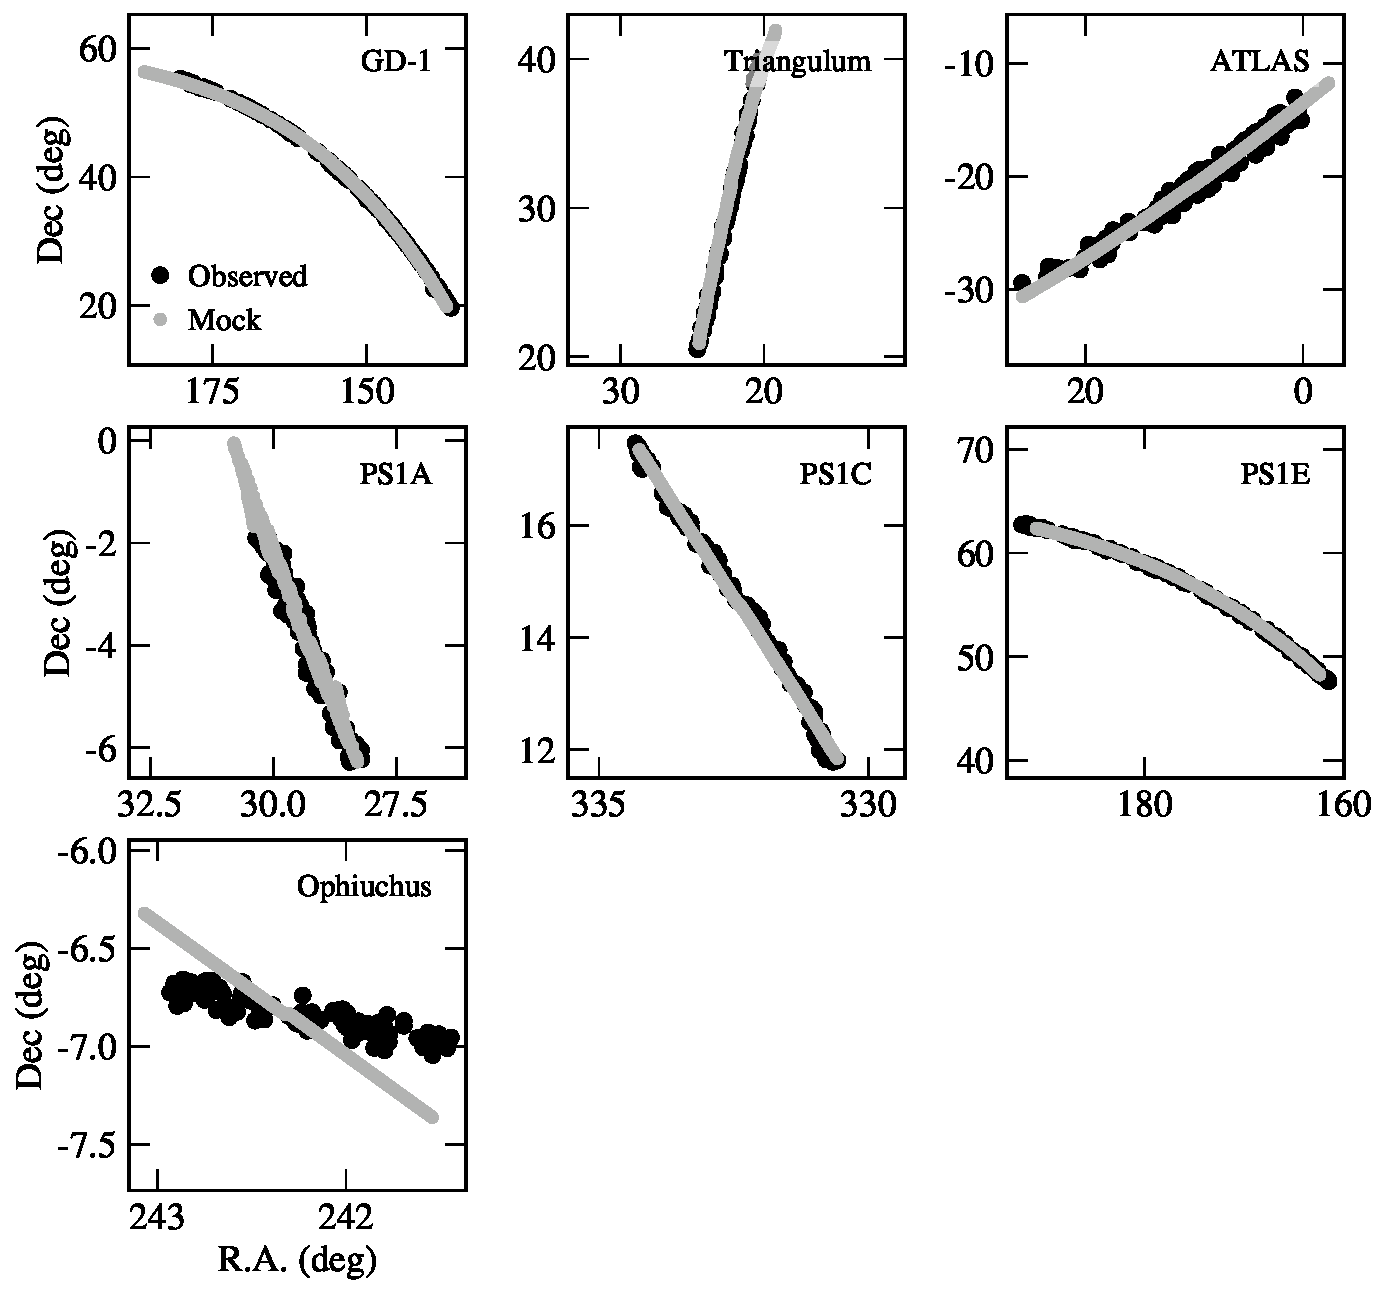
\includegraphics[width=\textwidth]{mocks.pdf}
\caption{On-sky positions of streams analyzed in this work, with one stream per panel, and the stream name in the upper right corner.
In each panel, the observed stream members are shown in black, whereas a best-fitting mock stream is plotted in gray.
All of the mock streams have been generated in the same gravitational potential, and they fit the observations reasonably well.
Streams where the mock deviates from observations likely experienced a different gravitational potential for at least a part of its evolution.
}
\label{fig:gallery}
\end{center}
\end{figure}

\section{Robust matrix inversion}
\label{sec:inversion}
Inverting a Fisher matrix is a core operation in calculating Cram\' er--Rao lower bounds and thus measuring the information content in stellar streams. 
Often, this problem is ill-conditioned, i.e. if the input Fisher matrix $I$ is modified only slightly, the standard numerical algorithms, such as that employed in \texttt{numpy.linalg.inv}, return a very different inverse $I^{-1}$.
We adopt an iterative approach of rescaling the problem to ensure a robust inverse is obtained, and outline it below.

Starting with a matrix $A$, which may have a large condition number, we are looking for a matrix $Q$, such that $Q A = I$.
If we have a guess for $Q$, and the guess is good, then the matrix $QA$ has a low condition number, and can be reliably inverted using the standard algorithm for numerical inversion.
Then it follows:
\begin{equation*}
(QA)^{-1} Q = A^{-1} Q^{-1} Q = A^{-1}
\end{equation*}
We have just obtained a better guess for the inverse of the original matrix $A$, and adopt it as the matrix $Q$ in the next iteration.
This procedure is repeated until $Q$ converges to $A^{-1}$, i.e., $Q A = I$ to machine precision.

In our current implementation, we use the standard, unreliable inverse as the starting guess $Q$. 
Convergence to the true inverse is typically obtained after several ($\lesssim2$) iterations.

\end{document}

